%% ===========================
\chapter{Bestimmung einer Datenbank}
\label{ch:AnalyseDatenbanken}
%% ===========================

Ein Ziel der Arbeit ist es kurze Antwortzeiten in der Beantwortung von Benutzeranfragen zu erreichen. Die maßgebende Komponente in diesem Fall ist die Datenbank. Sie führt die zeitintensiven Berechnungen des Gesamtsystems durch. Um Anhaltspunkte für mögliche Kandidaten zu bekommen, sollen im Folgenden eine Reihe bekannter Datenbanken vorgestellt und gegenübergestellt werden. Bei der Zusammenstellung wurde darauf geachtet, dass ein möglichst weites Spektrum unterschiedlicher Datenbanksysteme ausgewählt wurde.

%% ===========================
\section{Einzelbetrachtung von Datenbanken}
\label{ch:AnalyseDatenbanken:sec:Datenbanken}
%% ===========================

Im Folgenden werden nun einige Datenbanken vorgestellt. Dabei wird insbesondere versucht einen guten Überblick über die Charakteristika der einzelnen Datenbanken zu geben. Der dahinter stehende Gedanken ist, dass der Vergleich und die Auswahl von einer Datenbank dadurch besser nachvollziehbar werden. 

%% ===========================
\subsection{CouchDB}
\label{ch:AnalyseDatenbanken:sec:Datenbanken:subsec:CouchDB}
%% ===========================

CouchDB \cite{couch2013} ist eine dokumentorientierte Datenbank, die seit Anfang 2008 unter der  Apache-Lizenz verbreitet wird. In CouchDB werden die Daten in Collections anstatt in Tabellen abgelegt. Collections bestehen aus einer Sammlung von unabhängigen Dokumenten. Jedes Dokument verwaltet seine eigenen Daten in einem freien Schema. 
Ein Dokument in CouchDB kann Werte mit festen Datentypen (Text, numerisch oder boolean) oder Datenstrukturen (ein Dokument oder Liste) besitzen. In CouchDB werden für Indizes B-Bäume verwendet, sodass die Ergebnisse sortiert aufbewahrt und Wertebereichabfragen ausgeführt werden können. Abfragen können parallel über mehrere Rechner mit einem MapReduce Mechanismus verteilt ausgeführt werden. CouchDB erreicht Skalierbarkeit durch asynchrone Replikation\footnote{Wenn zwischen der Bearbeitung der Daten und der Replizierung eine Latenz liegt, spricht man von Asynchronität. Die Daten sind nur zu dem Zeitpunkt der Replikation synchron.} und nicht durch eine  Fragmentierung der Daten. Lesezugriffe können auf beliebigen Server stattfinden, wenn Aktualität keine Rolle spielt. Updates hingegen müssen an alle Server weitergegeben werden.

CouchDB kann wie andere NoSQL-Datenbanksysteme eine Eventual-Consistency der Daten bieten. Es implementiert MVCC auf einzelne Dokumente, mithilfe einer Sequenz-ID, die für jede Version eines Dokuments generiert wird. Eine Anwendung wird von CouchDB benachrichtigt wenn jemand anderes das Dokument aktualisiert hat, seitdem es zuletzt auf der Datenbank abgelegt wurde. Die Anwendung kann dann versuchen die Updates zu kombinieren (merge) oder das Update zu wiederholen, um die Daten zu überschreiben. CouchDB erfüllt außerdem im lokalen Einsatz die ACID-Eigenschaften, da jede Transaktion eine in sich abgeschlossene Operation, die entweder ganz oder gar nicht ausgeführt wird ist. Es treten keine Seiteneffekte zwischen den Anfragen auf.

%% ===========================
\subsection{MongoDB}
\label{ch:AnalyseDatenbanken:sec:Datenbanken:subsec:MongoDB}
%% ===========================

MongoDB ist ein in C++ geschriebener, Open Source Document Store \cite{books/daglib/0025185}. Es besitzt einige Ähnlichkeiten mit CouchDB. Beide bieten Indizes auf Collections und arbeiten mit einer optimistischen Synchronisation.

MongoDB speichert Daten in einem JSON-ähnlichen, binären Format namens BSON. BSON unterstützt boolean, integer, float, Datum, String-und Binär-Typen. Die Treiber der Clients wandeln die lokalen Dokumentdatenstrukturen in das BSON Format und senden diese an den MongoDB-Server. Weiterhin unterstützt MongoDB die GridFS-Spezifikation für große binär Dateien, wie z.B. Filme oder Bilder. MongoDB unterstützt Master-Slave-Replikation mit automatischem Failover und Recovery. Replikation (und Wiederherstellung) basieren auf dem Prinzip der Fragmentierung. Collections werden dabei automatisch fragmentiert. Die Replikation ist asynchron umgesetzt um höhere Leistung zu erzielen, jedoch können Updates dadurch bei einem Crash verloren gehen. 

%% ===========================
\subsection{Voldemort}
\label{ch:AnalyseDatenbanken:sec:Datenbanken:subsec:Voldemort}
%% ===========================

Projekt Voldemort \cite{vod2013} ist eine verteilte Key-Value-Store Datenbank (entwickelt von LinkedIn), welches ein hoch skalierbares Speicher-System zur Verfügung stellt. Voldemort repliziert sich durch automatisches Partitionieren und anschließendes Verteilen der Daten auf mehrere Server. Jeder Server stellt einen unabhängigen Knoten im System dar, der für die Verwaltung seiner Daten verantwortlich ist. Dadurch existiert kein Single Point of Failure im Cluster. Ein solches Daten Model erlaubt eine Cluster Expansion, ohne eine Neuverteilung der Daten vornehmen zu müssen. In Voldemort können verschiedene Storage Systeme, wie BerkeleyDB oder MySQL eingesetzt werden. 

Für die Ablage der Daten werden in Voldemort sogenannte Stores verwendet. Unterstützt werden lediglich Key-Value Ablagen. Allerdings können die Werte auch komplexe Datenstrukturen wie Maps oder Listen beinhalten. Voldemort stellt für die Datenmanipulation vier verschiedene Operatoren zur Verfügung:

\begin{itemize}

	\item PUT (Key,Value)
	\item GET (Key)
	\item MULTI-GET (Keys)
	\item DELETE (Key, Version) 

\end{itemize}

Eine Möglichkeit für Bereichsabfragen ist nicht vorhanden. Zur Gewährleistung der Eventual-Consistency werden Timestamps und Vektoruhren eingesetzt. Neben der Eventual-Consistency bietet Voldemort einen Betrieb mit starker Konsistenz an.       

%% ===========================
\subsection{Redis}
\label{ch:AnalyseDatenbanken:sec:Datenbanken:subsec:Redis}
%% ===========================

Redis \cite{red2013} ist ein In-Memory-, Key-Value-Store mit einer Option für Persistenz. Redis Datenmodell unterstützt Strings, Hashes, Listen, Mengen und sortierte Mengen. Obwohl Redis für In-Memory-Daten entworfen wurde, kann je nach Anwendungsfall ein (semi-) persistenter Bestand angelegt werden. Dieser wird durch die regelmäßige Ablage des Datenbestandes auf die Festplatte erreicht. Überdies werden durch Aufzeichnen eines Logs alle ausgeführten Operationen protokolliert, damit der Originalzustand bei Bedarf wiederhergestellt werden kann. Weiterhin kann Redis mit einer Master-Slave-Architektur repliziert werden. Genau wie andere Key-Value-Stores implementiert Redis insert, delete und lookup Operatoren. Weiterhin setzt Redis atomare Updates durch den Einsatz von Sperren um, die einen exklusiven Zugriff eines Prozesses auf eine Ressource realisieren. 

%% ===========================
\subsection{HBase} 
\label{ch:AnalyseDatenbanken:sec:Datenbanken:subsec:HBase}
%% ===========================

HBase ist eine verteiltes, Open Source Wide Column Store Datenbanksystem, welches auf Googles BigTable basiert \cite{Chang:2006:BDS:1267308.1267323}. HBase verwendet Apache Hadoop und Apache ZooKeeper  \cite{Hunt:2010:ZWC:1855840.1855851} und das Hadoop Distributed Filesystem (HDFS) \cite{Shvachko:2010:HDF:1913798.1914427}, um Skalierbarkeit und Replikation zu bieten. Zeilenoperationen sind in HBase atomar, mit Sperren auf Zeilenebene und Transaktionen. HBase wurde entwickelt um hohe Leistung für intensive Leseaufgaben zu erzielen.

Insbesondere stellt es lineare und modulare Skalierbarkeit, sowie streng konsistenten Datenzugriff und automatische, konfigurierbare Fragmentierung von Daten zu Verfügung. Auf Tabellen kann in HBase über eine Java-, Avro\footnote{Avro ist ein Remote Procedure Call- und Serialisierungs-Framework, das als Teil von Apaches Hadoop-Projekt entwickelt worden ist.}- oder Thrift-API zugegriffen werden. In Abbildung \ref{db_hbase} ist ein Beispiel zur Art der Datenhaltung in HBase dargestellt. Anwendungen speichern in HBase Daten in Tabellen, die aus Zeilen und Spalten-Familien bestehen. Spalten-Familien beinhalten wiederum Spalten. Darüber hinaus kann jede Zeile einen anderen Satz von Spalten beinhalten. Alle Spalten sind mit einem vom Benutzer bereitgestellten Schlüsselspalte indiziert und in Spalten-Familien gruppiert.

\begin{figure}[htbp]
\centering
  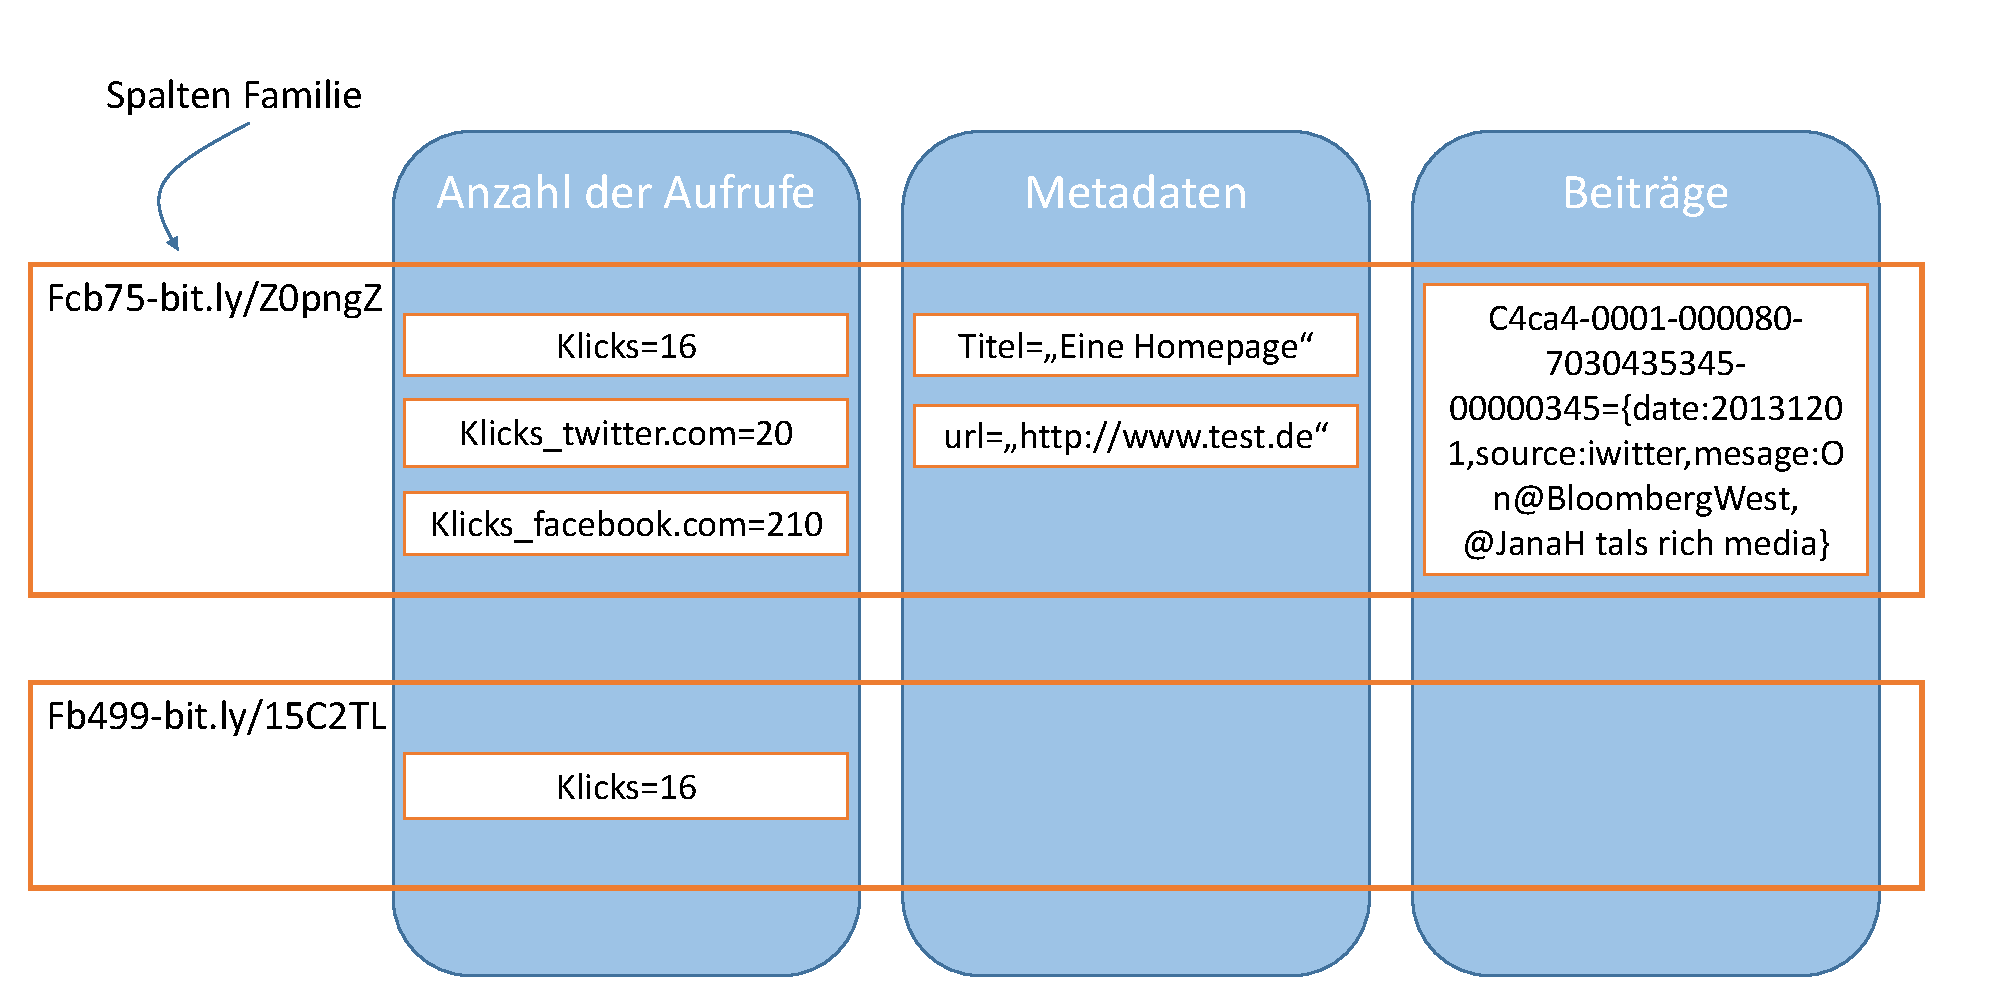
\includegraphics[width=1.0\textwidth, width=1.0\textwidth]{pics/HBase.pdf}
\caption{Komponenten des Systems und der Umwelt}
\label{db_hbase}
\end{figure} 

%% ===========================
\subsection{Cassandra} 
\label{ch:AnalyseDatenbanken:sec:Datenbanken:subsec:Cassandra}
%% ===========================
Apache Cassandra ist ein Wide Column Store der von Facebook entwickelt wurde \cite{Lakshman:2010:CDS:1773912.1773922}. Es ist eine Mischung aus Amazon Dynamo und Google BigTable, wodurch es des öfteren als Hybrid zwischen Key-Value-Store und Column Store bezeichnet wird. Der Verweis auf Amazon Dynamo beruht auf der Verwendung dessen Replikationsmechanismu der leicht weiterentwickelten wurde. Außerdem nutzt Cassandra die Datenstruktur von BigTable. Cassandra wurde entwickelt, um große Daten-Workloads über mehrere Knoten, ohne Single Point of Failure zu behandeln. Die Architektur ist von der Annahme geprägt, dass System-und Hardware-Fehler jederzeit auftreten können. Cassandra behandelt das Problem von Fehlern durch Verwendung eines Peer-to-Peer-System, in dem alle Knoten gleichberechtigt sind und die Daten über alle Knoten des Clusters verteilt werden. Jeder Knoten tauscht Informationen über das Cluster im Sekundentakt aus. In den Commit-Log werden zuallererst die Schreibvorgänge protokolliert bevor die Daten auf eine In-Memory Struktur (memtable) geschrieben werden. Sobald die Speicherstruktur voll ist werden die Daten in eine Datei (SSTable) auf der Festplatte abgelegt. Die durch Schreibvorgänge veränderten Daten werden automatisch aufgeteilt und auf mehrere Cluster repliziert. Weiterhin wurde Cassandra entwickelt um hohe Leistungen in schreibintensiven Aufgaben zu erzielen.

Cassandras Datenmodell basiert auf einem partitionierten Row-Store mit Eventual-Consistency. Zeilen werden in Tabellen organisiert, wobei die erste Komponente des Primärschlüssels einer Tabelle der Partitionschlüssel ist. Andere Spalten können getrennt vom Primärschlüssel indiziert werden. Was Cassandra von HBase unterscheidet sind ihre Spalten, die in einer verschachtelten Weise in Spalten-Familien gruppiert werden können. In der Abbildung \ref{db_cassandra} sind die Verschachtlungen dargestellt.

\begin{figure}[htbp]
\centering
  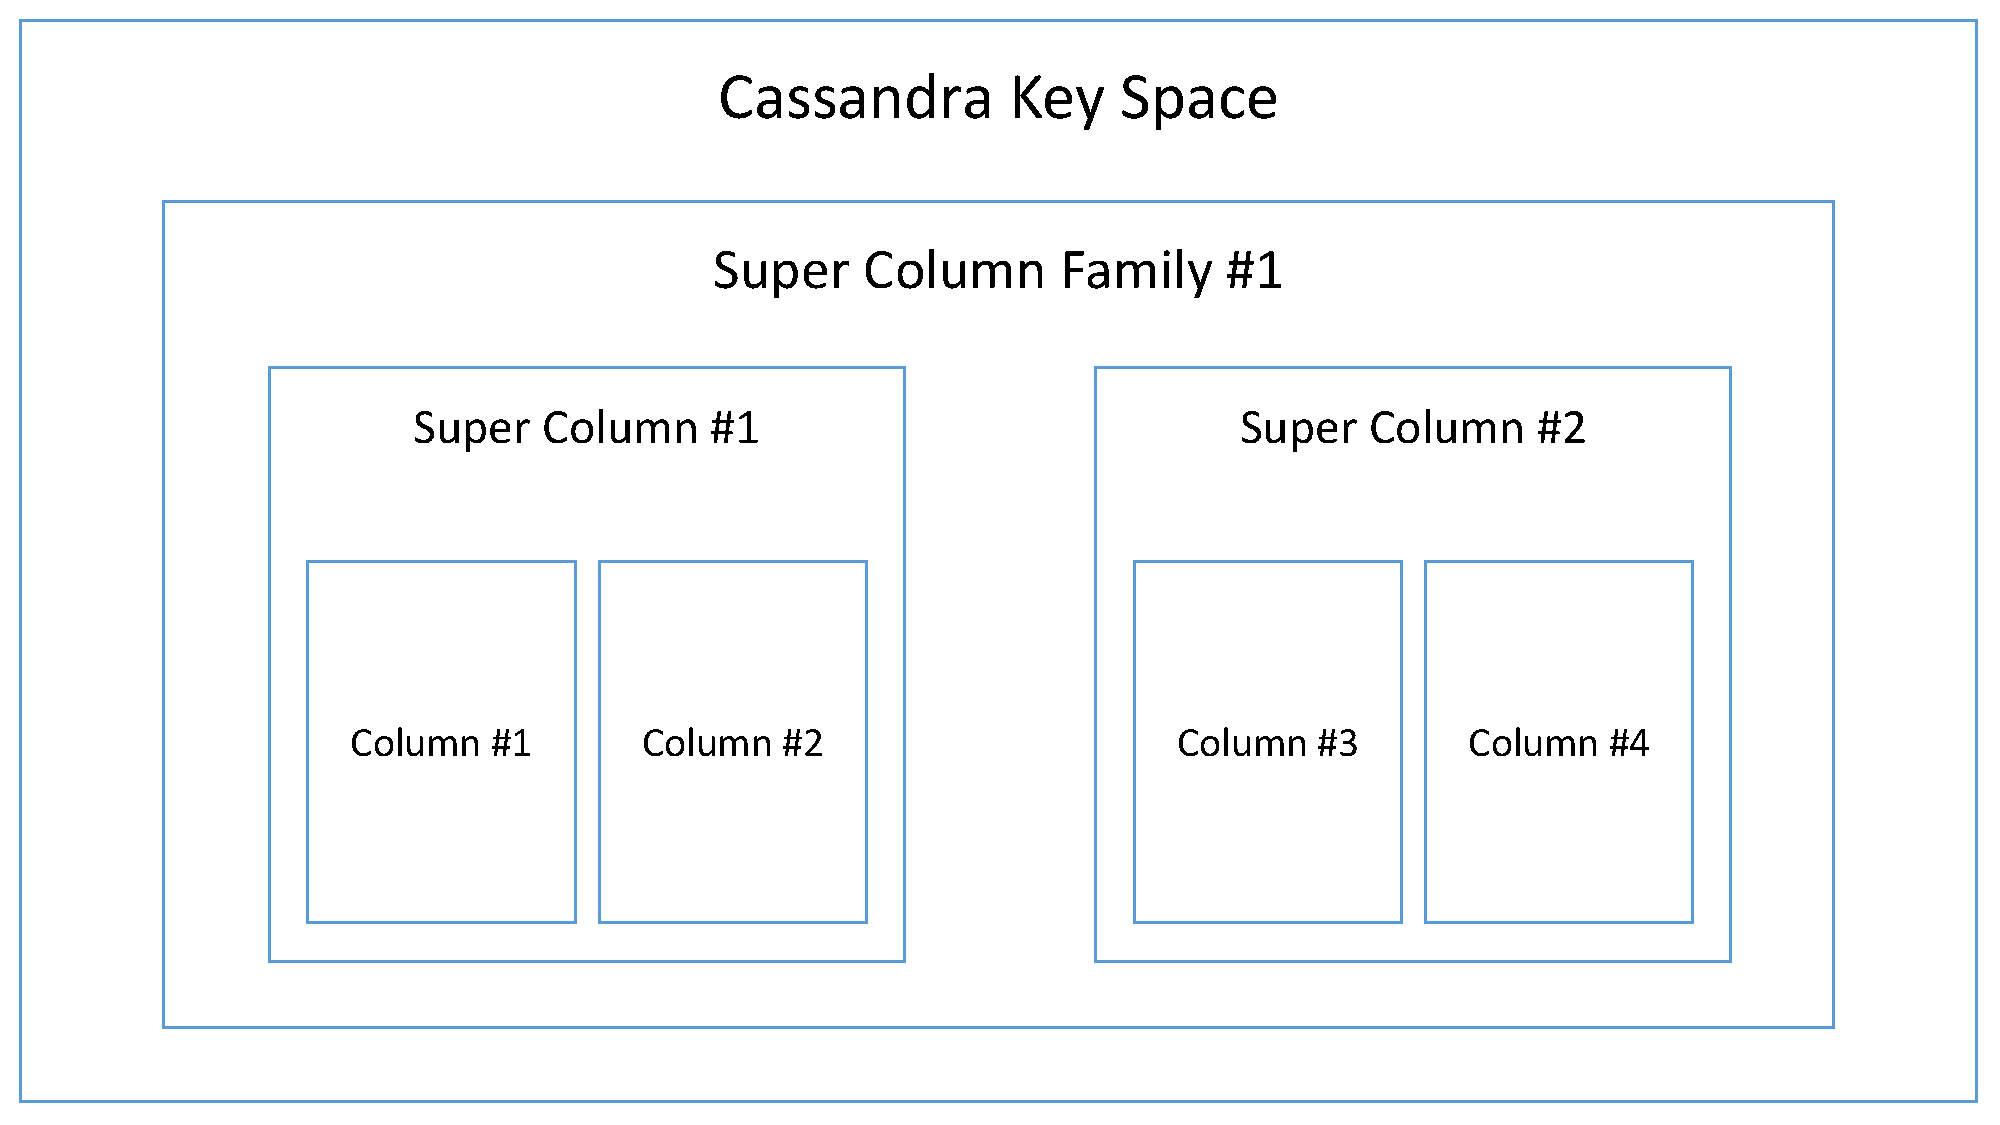
\includegraphics[width=0.8\textwidth, width=0.8\textwidth]{pics/cassandra.pdf}
\caption{Schematische Darstellung des Cassandra Datenmodells}
\label{db_cassandra}
\end{figure} 

%% ===========================
\subsection{VoltDB} 
\label{ch:AnalyseDatenbanken:sec:Datenbanken:subsec:VoltDB}
%% ===========================

VoltDB \cite{volt2013a} ist ein ACID-konformes, relationales In-Memory-Datenbanksystem, abgeleitet vom Forschungsprototyp H-Store \cite{kallman08}. Da VoltDB auf dem Ansatz der relationalen Algebra beruht und auf verteilten Knoten betrieben werden kann, zählt es zu den NewSQL-Datenbanken. Es basiert auf einer Shared-Nothing-Architektur und wurde entwickelt, um auf einem Cluster mit mehreren Knoten zu laufen. Erreicht wird dies indem die Datenbank in getrennte Partitionen aufgeteilt wird, bei dem jeder Knoten Besitzer und Verantwortlicher für die jeweiligen Partitionen ist. Die Anfragen in VoltDB werden seriell in einem einzigen Thread ausgeführt, sodass keine Sperren and Riegel innerhalb der Transaktionen mehr notwendig sind \cite{volt2013b}. Die Daten werden im Arbeitsspeicher gehalten, was eine Ausführung ohne Netzwerkzugriff und I/O-Vorgänge ermöglicht, falls die Daten nur auf einem Knoten liegen.  

%% ===========================
\subsection{H2} 
\label{ch:AnalyseDatenbanken:sec:Datenbanken:subsec:H2}
%% ===========================

H2 ist ein in Java geschriebenes relationales Datenbanksystem, dass im Jahre 2004 von Thomas Müller veröffentlicht wurde. Es wird unter der Eclipse Public License verbreitet und ist damit Open Source. H2 bietet neben den festplattenbasierten Tabellen, auch eine In-Memory Variante an. Tabellen können dabei dauerhaft oder temporär sein. Weiterhin beherrscht H2 referenzielle Integrität, Transaktionen, Clustering, Datenkompression, Verschlüsselung und SSL \cite{h2:2013}. Die Datenbank kann im Embedded- oder Server-Modus betrieben werden.

%% ===========================
\subsection{Neo4J} 
\label{ch:AnalyseDatenbanken:sec:Datenbanken:subsec:Neo4J}
%% ===========================

Neo4j ist eine in Java implementierte Open-Source-Graphdatenbank. Neo4j wird des öfteren als eine eingebettete, Disk-basierte, ACID-transaktionale Datenbank-Engine bezeichnet \cite{SWB-386976589}. Es speichert strukturiert Daten in Graphen anstatt in Tabellen. Für den Zugriff auf die Daten bietet Neo4J die Abfragesprache Cypher an. Cypher ist eine deklarative Graphabfragesprache, die es erlaubt  ausdrucksstarke und effiziente Abfragen und Aktualisierung des Graphen vorzunehmen. Überdies unterstützt Neo4J noch andere Zugriffskonzepte, die im Abschnitt \ref{ch:AnalyseDatenbanken:sec:Gegenüberstellung} erwähnt werden.

Im Neo4J Datenmodell wird alles durch Knoten, Beziehungen und Eigenschaften umgesetzt. Eine Beziehung verbindet zwei Knoten, hat einen klar definierten, verbindlichen Typ und kann wahlweise gerichtet sein. Eigenschaften sind Schlüsselwertpaare, die an Knoten und Beziehungen gebunden sind. In Abbildung \ref{db_neo4J} ist ein Beispiel modelliert.

\begin{figure}[htbp]
\centering
  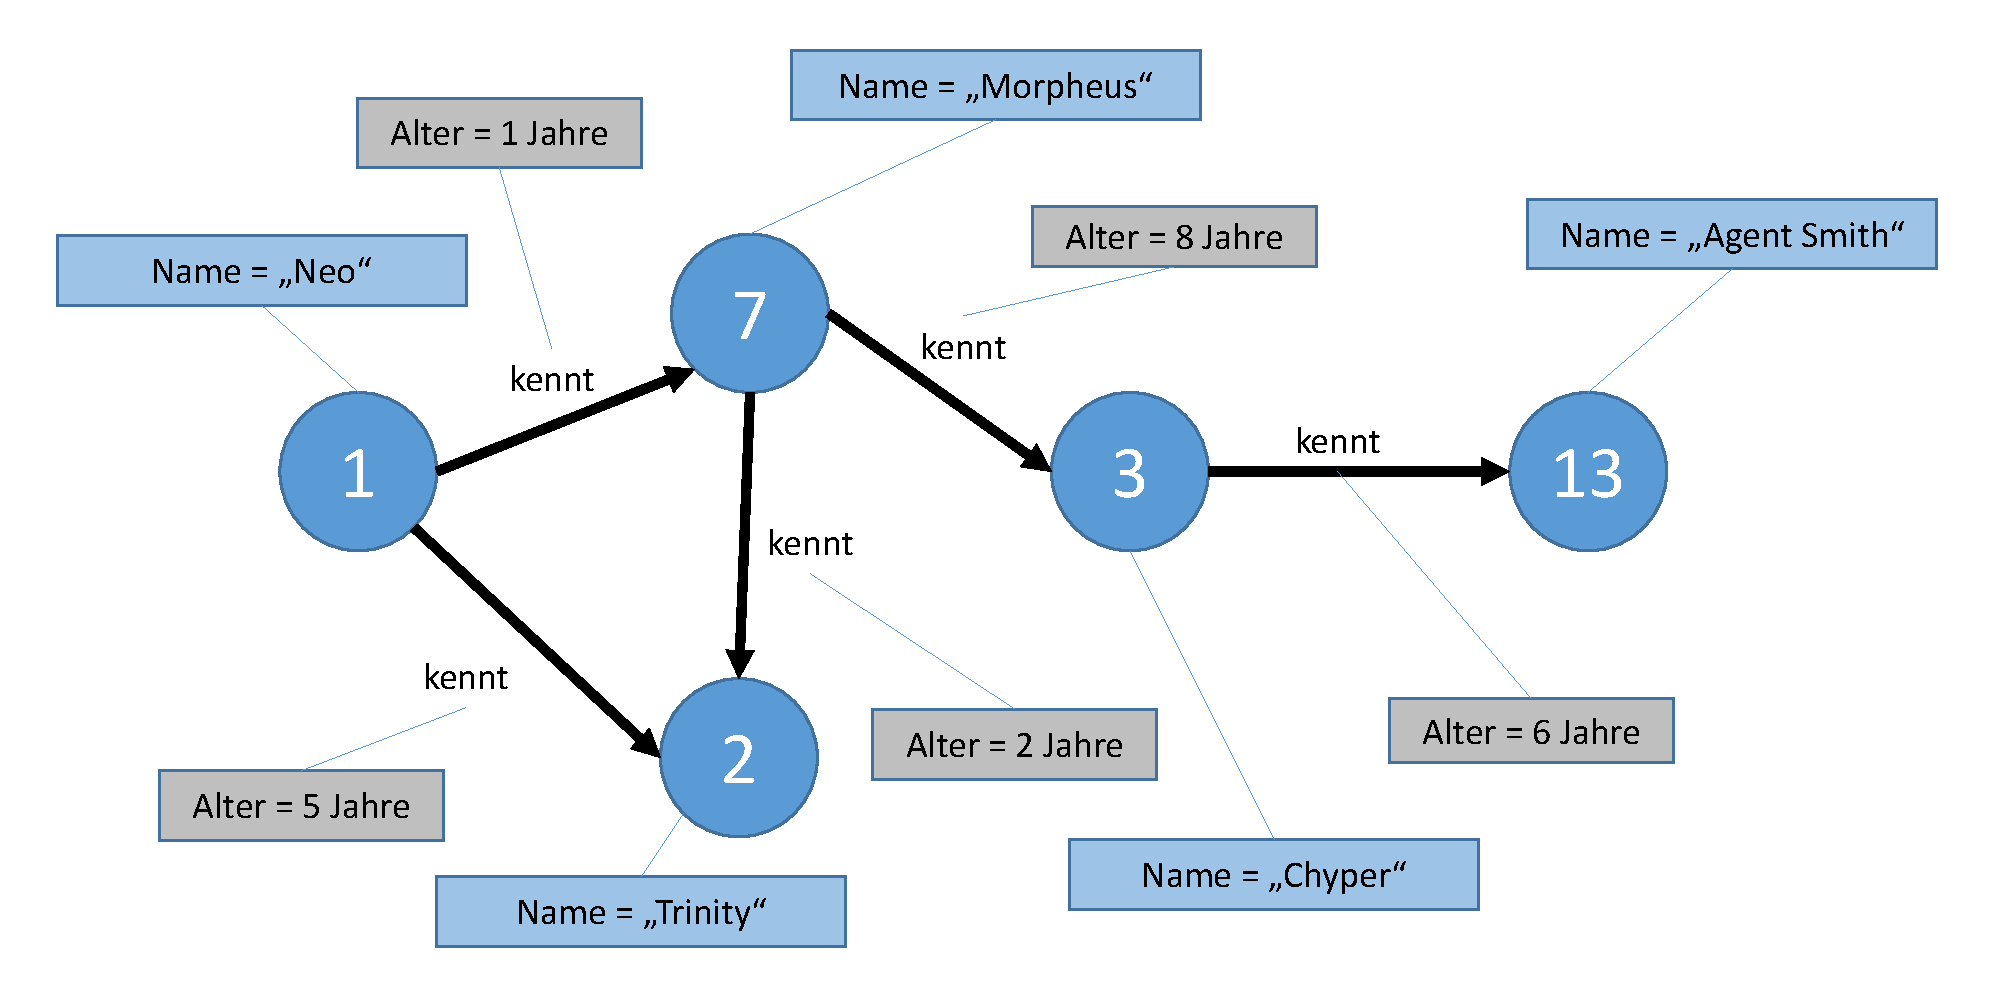
\includegraphics[width=0.9\textwidth, width=0.9\textwidth]{pics/neo4J.pdf}
\caption{Datenmodell anhand eines Social-Network-Beispiels}
\label{db_neo4J}
\end{figure} 

In der Abbildung besitzt jeder Knoten eine ID (Zahl) und jede Beziehung  einen Typ. Weiterhin existiert nur ein einziger Typ im Beispiel, mit der Bezeichnung "kennt". Das Beispiel besitzt Knoten mit der Eigenschaft (Name) und die Beziehungen verfügen über Eigenschaften zur Beschreibung wie lange sich die Personen bereits kennen. 

Typische Anwendungsbereiche von Neo4J sind beispielsweise Semantic Web, LinkedData, GIS, Genomanalysen und Modellierung von sozialen Netwerken.

%% ===========================
\section{Gegenüberstellung} 
\label{ch:AnalyseDatenbanken:sec:Gegenüberstellung}
%% ===========================

Zur übersichtlichen Gegenüberstellung der Datenbanken wird die Tabelle \ref{tb_charakteristika} herangezogen. Sie enthält vergleichbare Eigenschaften von Datenbanken, auf die im Folgenden eingegangen wird. 

Die erste Eigenschaft ist das Erscheinungsjahr einer Datenbank, welches bereits Rückschlüsse auf die Reife des Datenbanksystems in verschiedenen Aspekten ermöglicht. Ältere Datenbanken haben bereits viele ihrer anfänglichen Fehler beseitigt, was sie für den Einsatz in produktiven Umgebungen geeigneter machen. Natürlich sind ältere Systeme nicht gänzlich frei von Fehlern, allerdings existieren für viele Probleme entsprechende Lösungsansätze. Cassandra zum Beispiel, erhielt über die Jahre neben zahlreichen Bugfixes, MapReduce Support, sekundäre Indizies, verbesserte Komprimierung, eine eigne Query Sprache (CQL). Es gibt allerdings keine Regel die besagt zu welchem Zeitpunkt ein System die Reife für den produktiven Einsatz erreicht hat. Es spielen natürlich auch andere Faktoren bei der Bestimmung der Ausgereiftheit eine Rolle, wie z.B. die Größe des Unternehmens oder Teams das hinter der Datenbank steht. Die Eigenschaft hat weniger den Zweck eines Kriteriums, sondern eher eines Indikators. 

\begin{table}[H]
\tiny
\caption{Gegenüberstellung der Datenbankeigenschaften}
\label{tb_charakteristika}
\setlength{\tabcolsep}{1mm}
\begin{tabulary} {\linewidth} {C | C | C | C | C | C | C | C | C | C}
\toprule
Eigenschaft & HBase & Cassandra & CouchDB & MongoDB & Redis & Voldemort & VoltDB & H2 & Neo4j\\  
\midrule
Release Datum & 2008 & 2008 & 2005 & 2009 & 2009 & 2009 & 2010 & 2004 & 2007\\
\midrule
Datenbankmodell & Wide Column & Wide Column & Document & Document & Key-Value & Key-Value& Relational DBMS & Relational DBMS & Graphdatenbank\\
\midrule
Lizenz & Open Source & Open Source & Open Source & Open Source & Open Source & Open Source & Kommerziell & Open Source & Open Source\\
\midrule
Server Betriebssysteme & Linux, Unix, Windows & BSD, Linux, OS X, Windows & Android, BSD, Linux, OS X, Solaris, Windows & Linux, OS X, Solaris, Windows & BSD, Linux, OS X, Windows & Linux, Unix, Windows & Linux, OS X & plattformunabhängig & Linux, OS X, Windows\\
\midrule
Daten-schema & schemafrei & schemafrei & schemafrei & schemafrei & schemafrei & schemafrei & ja & ja & schemafrei\\
\midrule
Typisierung & nein & ja & nein & ja & nein & nein & ja & ja & ja\\
\midrule
Sekundärindizes & nein & eingeschränkt & ja (über Views) & ja & nein & nein & ja & ja & ja\\
\midrule
SQL & nein & nein & nein & nein & nein & nein & ja & ja & nein\\
\midrule
APIs und andere Zugriffskonzepte & Java API, RESTful HTTP API, Thrift & Proprietäres Protokoll (CQL) & RESTful HTTP/JSON API & Proprietäres Protokoll basierend auf JSON & Proprietäres Protokoll & Proprietäres Protokoll & Java API, RESTful HTTP/JSON API, JDBC & Java API, ODBC, JDBC & Cypher query language, Java API, RESTful HTTP API\\
\midrule
Unterstützte Programmiersprachen & C, C\#, C++, Groovy, Java, PHP, Python, Scala & C\#, C++, Java, Perl, PHP, Python, Ruby, +5 & C, C\#, Java, JavaScript, Perl, PHP, PL/SQL, Python, Ruby, +9 & C\#, C++, Java, JavaScript, Perl, PHP, Python, Ruby, +4 & C\#, C++, Java, JavaScript, Perl, PHP, Python, Ruby, +12 & C\#, C++, Java, Perl, PHP, Python, Ruby, +8 & C\#, C++, Java, PHP, Python & C\#, C++, Java, PHP, Phyton & .Net, Clojure, Go,  Groovy, Java, JavaScript, Perl, PHP, Python, Ruby, Scala \\
\midrule
MapReduce & ja & ja & ja & ja & nein & nein & nein & nein & nein\\
\midrule
Konsistenzkonzept & Immediate Consistency & Eventual Consistency, Immediate Consistency & Eventual Consistency & Eventual Consistency, Immediate Consistency & Eventual Consistency & Strict Consitency, Eventual Consistency &  Integritätsbedingungen & Integritätsbedingungen & Eventual Consistency\\
\midrule
Transaktionskonzept & nein & nein & nein & nein & optimistisches Locking & nein & ACID & ACID & ACID\\
\midrule
Nebenläufigkeit & ja & ja & ja & ja & ja & ja & ja & ja & ja\\
\midrule
Embeddable & nein & ja & ja & nein & nein & ja & ja & ja & ja\\
\midrule
In Memory fähig & nein & nein & nein & nein & ja & hybrid & ja & ja & nein\\
\bottomrule
\end{tabulary}
\end{table}

Ein wichtiger Faktor ist die Lizenz unter der die Datenbank vertrieben wird. Für Unternehmen ist die Wirtschaftlichkeit eines Produktes von immenser Bedeutung. Deshalb bieten Open Source Produkte mit ihren geringen Anschaffungskosten einen hohen Anreiz. Bei der Verwendung von Open Source ist allerdings mit einem schwächeren Support als bei kommerziellen Produkten zu rechnen. Ein weiteres Argument zur Nutzung von Open Source ist die Möglichkeit einen Einblick in den Quelltext zu erhalten und diesen gegebenenfalls auch zu bearbeiten. Kommerzielle Lizenzen bieten hingegen eine höhere Zukunftssicherheit als Open Source Produkte, da Unternehmen in ihrer Arbeit beständiger sind als Privatpersonen.

Die Betrachtung von unterstützten Programmiersprachen und Betriebssysteme ist zum Feststellen der Kompatibilität mit vorhandenen Systemen notwendig. In Unternehmen sollte idealerweise schon Erfahrung in den potenziellen Technologien vorhanden sein. Denn externe Mitarbeiter, sowie Schulungen sind teuer und sollten bei der Wahl einer Technologie oder Produktes berücksichtigt werden. 

Datenbanken können ein festes Schema besitzen oder schemafrei sein. Welche der beiden Möglichkeiten für die Lösung einer Problemstellung geeigneter ist kann anhand der Struktur der abzulegenden Daten bestimmt werden. Wenn sich die Struktur der abzulegenden Daten häufig ändert oder keine einheitliche Struktur unter den Daten zu erkennen ist, sind schemafreie Datenbanken von Vorteil. Denn sie bieten ein hohes Maß an Flexibilität, wohingegen durch die Nutzung eines Schemas eine bessere Kontrolle über die Daten entsteht.  

Sekundärindizes können Lesegeschwindigkeiten steigern, weshalb sie zum Erreichen von kurzen Antwortzeiten eine interessante Datenbankenfunktion darstellen. Sie erlauben Indizes auf einem oder mehreren Schlüsseln oder Nicht-Schlüsselattributen, wodurch die Effizienz einer Suche gesteigert werden kann. Einige NoSQL-Datenbanken unterstützen solche Indizes, wohingegen relationale Datenbanksysteme die Definition beliebiger Sekundärindizes gestatten. 

Die Vermeidung von Laufzeitfehlern ist ein Ziel der Typisierungen. Typisierte Datenbanken schränken den Wertebereich von Variablen ein. Ein Vorteil der dadurch entsteht ist eine Vorabkontrolle der Daten, sodass nur Daten mit den entsprechenden Eigenschaften verwendet werden. Ein Nachteil ist die mangelnde Flexibilität. Der Entwickler muss sich wie beim Schema zwischen Flexibilität und Kontrolle entscheiden. 

Das in der Datenbank verwendete Zugriffskonzept spielt bei der Architektur des gesamten Systems eine Rolle. Zu einem ist zu unterscheiden ob es sich um ein proprietäres Protokoll oder ein standardisiertes Protokoll handelt. Proprietäre Protokolle weisen meist eine höhere Einarbeitungszeit für die Mitarbeiter auf. Bei der Arbeit mit Standardtechnologien kann auf vorhandenem Wissen aufgebaut werden, was die Einarbeitungszeit verkürzt. 

Eine Entscheidung hinsichtlich der Stärke von Konsistenz wird durch den Anwendungsfall bestimmt. Wenn die Redundanz von Daten kein Problem im Anwendungsfall darstellt ist keine hohe Konsistenz notwendig. Allerdings sollte die nächst höhere Anwendungsschicht bei Inkonsistenz damit rechnen, sonst kann es zu schwerwiegenden Fehlern kommen. 

Das Transaktionskonzept (Nebenläufigkeit) gibt an, ob gleichzeitig ausgeführte Datenmanipulationen durch die Datenbank unterstützt werden. Genau wie bei der Konsistenz ist der Anwendungsfall für die Wahl des Transaktionskonzeptes ausschlaggebend.   

Datenbanken die im Embedded-Modus betrieben werden können sehr einfach in Anwendungen integriert werden. Ein Vorteil dabei ist das es zu keinen Verzögerungen durch Netzwerkzugriffe kommt. 

%Außerdem besteht können die Datenbank und die Anwendung über Interprozesskommunikation Daten übertragen. 

Die CAS Software AG wünscht sich hohe Ausführungsgeschwindigkeiten, wodurch die In-Memory-Fähigkeit einer Datenbank von entscheidender Bedeutung sein kann.

%% ===========================
\section{Auswahl einer Datenbank}
\label{ch:AnalyseDatenbanken:sec:Ergebniss}
%% ===========================

Jede Datenbank hat ihre eigenen Stärken und Schwächen. Bei der Wahl einer geeigneten Datenbank ist nicht entscheidend welche Datenbank für allgemeine Aufgaben die optimale ist. Es ist wichtiger, dass die entsprechende Datenbank die Charakteristika die zur Erreichung des Ziels benötigt werden besitzt.

In dieser Arbeit steht eine geringe Antwortzeit als Eigenschaft der Datenbank im Vordergrund. Die Verwendung des Hauptspeichers als Speichersystem bedeutet einen theoretischen Geschwindigkeitsvorteil um circa 50.000 \cite{SWB-394434307}.
Das Speichersystem alleine ist zwar nicht aussagekräftig genug um die Entscheidung nur aus diesem Grund zu treffen. Es wird allerdings angenommen das simple Abfragen, die hauptsächlich Daten lesen, um einiges schneller sind als in festplattenbasierten Datenbanken. Fünf Datenbanken bieten diese Eigenschaft nicht. Deswegen ist zu untersuchen, ob diese Datenbanken andere Charakteristiken aufweisen können, die den Nachteil ausgleichen.

Cassandra und HBase ermöglichen hohe Performance durch horizontale Skalierung. Horizontale Skalierung ist vor allem bei hohem Datenaufkommen sinnvoll. Die Kunden der CAS Software AG sind alles mittelständische Unternehmen, welche nicht an die Nutzerzahlen von Facebook und Google herankommen. Daher sind keine täglichen Zugriffszahlen im Millionenbereich zu erwarten. Horizontale Skalierung ist dementsprechend nicht notwendig, sowie durch die Limitierung auf einen Rechner nicht möglich. Außerdem ist zu erwarten das Cassandra und HBase auf einzelnen Servern nicht an die Performance von In-Memory fähigen Datenbanken herankommen. Aufgrund dessen wurde sich gegen die beiden Vertreter der Wide Column Stores entschieden.

Die Document Store Datenbanken sind zwar auch horizontal skalierbar, jedoch kann wie bereits geschildert dieser Vorteil nicht ausgenutzt werden. Ihre Stärke liegt in ihrer Schema freien Datenhaltung, die an dieser Stelle von geringem Wert ist, da die verwendeten Daten eine feste Struktur besitzen. Außerdem werden Funktion wie \textit{SUM()} nicht in der Datenbank eigenen API mitgeliefert, was sie für analytische Aufgaben bedingt brauchbar macht. Letztendlich können CouchDB und MongoDB keine Argumente liefern, weshalb sie für unser Szenario geeignet sind. Infolgedessen entschied man sich gegen sie.

Die Key-Value-Stores ermöglichen niedrige Zugriffszeiten mit ihrer In-Memory Datenhaltung. Was ihnen zum Nachteil ausgelegt werden kann, ist ihre mangelnde Komplexität. Damit ist gemeint, dass man auf komplexe Suchalgorithmen oder Indizes verzichten muss, da der Zugriff auf einen Datensatz lediglich über dessen Schlüssel erfolgt. Weiterhin sind sie auf Punkt-Abfragen ausgelegt. Komplexe Abfragen können daher nur in der Logikschicht realisiert werden. Diese würde zu einer nicht vorhersehbaren Steigerung im Aufwand bei der Umsetzung der Datenbankzugriffsschicht führen. Viele Funktionen müssten vom Entwickler selbst implementiert werden. Daher wurde sich auch gegen die Key-Value-Stores entschieden. 

Neo4J wird bereits in vielen Bereichen eingesetzt und hat sich als robustes Produkt erwiesen. Weiterhin besitzt es Anbindungen an eine Reihe von Sprachen als auch Integrationsmöglichkeiten in vorhandene Frameworks wie Spring, Ruby on Rails, PHP, etc. Die Open-Source Lizenz ist natürlich auch ein Pluspunkt. Gerade in Anbetracht unseres Szenarios sind Graphen auf den ersten Blick eine sehr nützliche Form um Beziehungen zu ermitteln. Es muss allerdings beachtet werden, dass keine komplexen Verknüpfungen über viele Personen hinweg zu ermittelt sind. Es wären immer nur sehr wenige Kanten zu betrachten. Die Geschwindigkeitsvorteile von Graphdatenbanken lassen sich allerdings nur bei komplexen und weitreichenden Ermittlungen ausnutzen. Die Verwendung der Datenbank ist zwar eine Möglichkeit, jedoch kann sie ihre Stärken in dem für die Arbeit betrachtetem Szenario nicht richtig ausnutzen. Überdies sind kurze Antwortzeiten sehr wichtig und Neo4J bietet keine Funktionen zum Betrieb im Hauptspeicher. Es wäre lediglich mithilfe der Manipulation des Caches möglich einen In-Memory artigen Betrieb der Datenbank zu erreichen. Welche Seiteneffekt dabei auftreten ist nicht klar sowie die Probleme die dadurch entstehen könnten. Aufgrund dessen das keine komplexen oder weitreichenden Verknüpfungen zwischen vielen Personen betrachtet werden und sie Nachteile in der Latenz gegenüber In-Memory-Datenbanken haben, konnte Neo4J nicht überzeugen.

VoltDB ist von den Eigenschaften her ein optimaler Kandidat, allerdings nicht Open Source. Aufgrund dessen wurde sich gegen VoltDB entschieden. 

Die H2-Datenbank hingegen ist Open Source und bietet Optionen zum 
Vorhalten der Daten im Hauptspeicher. Davon werden sich hohe Geschwindigkeitsvorteile gegenüber herkömmlichen relationalen Datenbanksystemen erhofft. Durch den Ansatz der relationalen Algebra in der Datenbank ist die Arbeit mit SQL möglich. Das birgt Vorteile, da auf bereits bekanntem Wissen aufgebaut werden kann. Die H2-Datenbank wurde ausgewählt, da sie mit der Kombination von neuen Ansätzen wie der Nutzung des Hauptspeichers und alt bewährten Prinzipien aus der relationalen Algebra eine schlüssige Lösung ergibt.